
\part{Funcionales lineales}

\chapterimage{Pictures/0001} % Chapter heading image

\chapter{Funcionales lineales}

\section{Ejercicios y Teoremas}

\begin{definition}
Sea $V$ un espacio vectorial sobre $\mathbb{F}$. Entonces, una transformación lineal $$f:V\mapsto\mathbb{F}$$ es un funcional lineal sobre $V$. 
\end{definition}

\begin{exercise}
Sean $\alpha_1,...,\alpha_n \in\mathbb{R}$. Definimos:
$$\Phi:\mathbb{R}^n\mapsto\mathbb{R}\ni$$
$$\Phi(x_1,...,x_n)=\alpha_{1}x_{1}+...+\alpha_{n}x_{n}$$
$\Rightarrow\Phi$ es funcional lineal. 
\end{exercise}
\begin{notation}
$$f:\mathbb{R}^2\mapsto\mathbb{R}\ni$$
$$\Phi(x,y)=2x-y$$
\end{notation}

\begin{exercise}
Sea $C[0,1]$ un conjunto de funciones continuas en [2,1] y considere:
$$T:C[0,1]\mapsto\mathbb{R}\ni$$
$$T(g)=\int^1_0 g(x)dx$$
Nótese si $f,g\in[0,1]$ y $\alpha\in R$$\Rightarrow T(\alpha f+g)=\int^1_0[\alpha f+g](x)dx=\int^1_0[(\alpha f)(x)+g(x)]dx=\alpha\int^1_0f(x)dx+\int^1_0f(x)dx+\int^1_0 g(x)dx=\alpha T[f]+T[g]\Rightarrow$ es lineal $\Rightarrow$ T es funcional lineal. 
\end{exercise}

\begin{exercise}
Sea $$d:\mathbb{R}^{nxn}\mapsto\mathbb{R}\ni$$
$$d(A)=\text{determinante de A}$$
Recordar que: $$det(A+B)\neq det(A)+det(B)$$
$$det(\alpha A)\neq \alpha det(A)$$
$$d(A) \text{ no es funcional lineal}$$
\end{exercise}

\begin{exercise}
Sea $$T:\mathbb{R}^{nxn}\mapsto\mathbb{R}\ni$$
$$T(A)=\text{ traza de A}$$
$$\text{Si } A=[a_{ij}]\Rightarrow Tr(A) = \sum^n_{i=1}a_{ij}$$
$$\Rightarrow Tr(A) \text{ es funcional lineal.}$$
\end{exercise}
\begin{exercise}
Sea $V$ el espacio de todas las funciones sobre $\mathbb{R}$.
Definimos $$C_t: V\mapsto\mathbb{R}\ni$$
$$C_t(f)=f(t)\text{ , donde t es un número fijo.}$$
Nótese que:
\begin{enumerate}
    \item Sea $f,g\in V\Rightarrow L_t[f+g]=(f+g)(t)=L_t(f)+L_t(g)$
    \item Sea $\alpha\in\mathbb{R}\mapsto L_t(\alpha f)=(\alpha f)(t)=\alpha f(t)=\alpha L_t(f)\Rightarrow\text{ Es funcional lineal.}$
\end{enumerate}
\end{exercise}

\begin{notation}
Considere el funcional lineal $$f:\mathbb{R}^n\mapsto\mathbb{R}\ni$$$$f(x_1,...,x_n)=\alpha_1 x_1+...+\alpha_n x_n.$$
$$ \alpha_1\in\mathbb{R}$$ (fijos)
Sea $B=\{e_1,...,e_n\}$ la base usual de $\mathbb{R}^n$ y sea $B'=\{1\}$ la base usual de $\mathbb{R}$. $$f(1,0,...,0)=\alpha_1(1)+\alpha_2(0)+...+\alpha_1(0)$$
$$=\alpha_1$$
$$f(0,1,0,...,0)=\alpha_2$$
$$\vdots$$
$$\Rightarrow[f]^{B'}_B =[\alpha_1\,\alpha_2\,...\,\alpha_n]$$

\end{notation}

\begin{notation}
Si $f$ son funcionales lineales. 
$$f\in f[V,\mathbb{F}]\text{ si dim(V)=n}$$
$$\Rightarrow dim( f[V,\mathbb{F}])= n\cdot1=n$$
\end{notation}

\begin{definition}[$V^{*}$]
Al espacio de funciones lineales de V es $\mathbb{V}$ es $\mathbb{F}$ se le llama al espacio dual de $V$.
\end{definition}

\begin{notation}
Si $dim(V)=n \Rightarrow dim(V^*)=n$
\end{notation}

\subsection{Teorema}
\begin{theorem}
Sea $V$ un espacio vectorial finito dimensional y $B=\langle v_1,...,v_n\rangle$ una base ordenada de $V$. Entonces, existe una base: $B^* = \{\Phi_1,...,\Phi_n\}$ de $V^*$, tal que: 
$$\Phi_i(V_j)=
    \begin{cases} 
      1 & i=j \\
      0 & i\neq j  
   \end{cases} = \delta_{ij} $$
$$\Phi_i(V_j)=\delta_{ij}\xleftarrow{\text{ Delta de Kronecker}}$$


\end{theorem}

\subsection{Ejercicio}
\begin{exercise}
Considere la base de $\mathbb{R}^2$,
$$B=\{(2,1),(3,1)\}$$
entonces, encuentre una base para para $(\mathbb{R^2})^{*}\xleftarrow{\mathcal{L}[\mathbb{R}^2,\mathbb{R}^2]}$
\end{exercise}

\textbf{Solución:}
\begin{align}
    B^* &= \{\phi_1,\phi_2\} & \text{es tal que:}\\
    \intertext{Debemos encontrar $\alpha_1,\alpha_2,\beta_1,\beta_2$}
    \phi_1(x,y)&=\alpha_1 x+\alpha_2 y\\ 
    \phi_2(x,y)&=\beta_1 x+\beta_2 y\\
    \intertext{Encontramos $\alpha_1 y \alpha_2$:}
    \phi_1(v_1)&=\phi(2,1)=2\alpha_1+\alpha_1=1  & \delta_{11}\\
    \phi_1(v_2)&=\phi(3,1)=3\alpha_1+\alpha_2=0  & \delta_{11}\\
    \implies &\alpha_1=-1, \alpha=3\\
    \implies & \phi_1(x,y)=-x+3y\\
    \intertext{Encontramos $B_1,B_2$:}
    \phi_2(v_1)=\phi_2(2,1)= 2\beta_1+\beta_2 =0\\ 
    \phi_2(v_2)=\phi_2(3,1)= 3\beta_1+\beta_2 =1\\
    \implies & \beta_1=1,\beta_2=-2\\
    \implies &\phi_2(x,y) =x -2y 
\end{align}
$\implies$ La base dual de $B$, denotada por $B^*$ (i.e. la base del espacio dual $V^)*$, es \\$B^{*}=\{-x+3y,-x+2y\}$

\subsection{Ejercicio}
\begin{exercise}
Dada la base de $\mathbb{R}^3$:\\
$$B=\{(1,-1,3),(0,1,-1),(0,3,-2)\},$$
encuentre la base dual de $B^*$ (i.e. la basa para $\mathcal{L}[\mathbb{R}^3,\mathbb{R}]$)
\end{exercise}


\begin{align}
    \phi_1(x,y,z)&=\alpha_1 x +\alpha_2 y+\alpha_3 z\\
    \phi_2(x,y,z)&=\beta_1 x +\beta_2 y+\beta_3 z\\
    \phi_3(x,y,z)&=\gamma_1 x +\gamma_2 y+\gamma_3 z\\
    \intertext{Encontramos $\alpha_1,\alpha_2,\alpha_3$: }
    \p_1(v_1)&=\p_1(1,-1.3)=\al_1-\al_2+2\al_3=1\\
    \p_2(v_2)&=\p_1(0,1,-1)=0\al_1+\al_2 -1\al_3=0\\
    \p_3(v_3)&= \p_1(0,3,-2)=0\al_1+3\al_2-2\al_3=0\\
    \implies &\al_1=1,\al_2=\al_3=0 \implies \p_1(x,y,z)=x
    \intertext{Encontramos $\be_1,\be_2,\be_3$:}
    \p_2(v_1)&=\p_2(1,-1,3)=1\be-1\be+2\be= 0\\
    \p_2(v_2)&=\p_2(0,1,-1)=0\be+1\be-1\be= 1\\
    \p_2(v_3)&=\p_2(0,3,-2)=0\be+3\be-2\be= 0\\
    \implies &\be_1=7,\be_2=-2,\be_3=-3 \implies \p_2(x,y,z)=7x-2y-3z
    \intertext{Encontramos $\g_1,\g_2,\g_3$}
    \p_3(v_1)&=\p_3(1,-1,3)=1\g-1\g+2\g= 0\\
    \p_3(v_2)&=\p_3(0,1,-1)=0\g+1\g-1\g= 1\\
    \p_3(v_3)&=\p_3(0,3,-2)=0\g+3\g-2\g= 0\\
    \implies &\g_1=2,\g_2\g_3=1 \implies \p_3(x,y,z)=-2x+y+z
    \intertext{Por lo tanto:}
    B^* &= \{x,7x-2y-3z,-2x+y+z\}
    \intertext{Por otra parte, es necesario probar que $B^*$ es linealmente independiente}
    \text{Considere: }& \up_1\p_1+\up_2\p_2+...+\up_n\p_n =0\\
    \text{A probar: }& \up_1=\up_2=...=\up_n=0\\
    \intertext{Sea $v_i\in B$, $1\leq i\leq n$}
    \implies & (\up_1\p_1+...+\up_1\p_i+...+\up_n\p_n)(v_i)=0(v_i)\\
    \implies & \up_1\p_1(v_i)+...+\up_1\p_i(v_i)+...+\up_n\p_n)(v_i)=0\\
    \implies & 0+1 +0 &= 0\\
    \implies &\up_1=\up_2=...=\up_n=0 \implies \{\p_1,...,\p_n\}\text{ es linealmente independiente}\\
\end{align}

\subsection{Teorema}
\begin{theorem}
Sea $V$ un espacio vectorial finito dimensiona y sea $B=\{x_1,...,x_2\}$ una base ordenada para $V$. Entonces existe una base $B^* = \{\p_1,...,\p_n \}$ para $V^* \ni$ $$\p_i(x_j)=\delta_ij$$
Además, 
\begin{align}
    \intertext{(i) $\forall \p \in V^*$ se tiene:}\\
    \p =\p(x_1)\p_1+\p(x_2)\p_2+...+\p(x_n)\p_n\\
    \intertext{(ii) $\forall x \in V$ se tiene que:}\\
    x=\p_1(x)x_1+\p_2(x)x_2+...+\p_n(x)x_n\\
\end{align}
\end{theorem}

\begin{proof}
\begin{align}
    \intertext{A probar: $B^*$ es linealmente independiente. Considere:}\\
    \al_1\p_1+...+\al_n\p_n &=0_n \\
    \text{funcional lineal} &= \text{funcional lineal}\\
    \intertext{Aplicando a $x_i (i=1,...,n)$}\\
    (\al_1\p_1+...+\al_i\p_i+...+\al_n\p_n)(x_j)\\
    \implies \alpha_1\p_1(x_i)+...+\alpha_i\p_i(x_i)+...+\al_n\p_n(x_i)=0\\
    \implies \alpha_i =0  \\
    \implies B^* \text{ es linealmente independiente.}
    \intertext{(2)$B^*$ genera a $V^*$}
    \intertext{Sea $\phi\in v^*$. Entonces, sean:}
    \p(x_1)=\la_1,\p(x_2)=\la_2,...,\p(x_n)=\la_n\\
    \intertext{Por otro lado, hagamos:}
   \sigma = \la_1\p_1+\la_2\p_2+...+\la_n\p_n\\
   \implies \sigma(x_1) &= (\la_i\p_1+...+\la_n\p_n)(x_1)\\
    &= \la_1\p_1(x_1)+\la_2\p_2(x_1)+...+\lambda_n\p_n (x_1)\\ 
   &= \la_1 + 0+0\\
    \intertext{De la misma forma: }
    \sigma(x_i)=\la_i\\
    \implies \p(x_i)=\sigma(x_i) \\
   \implies \p = \sigma=\la_1\p_1+\la_2\p_2+...+\la_n\p_n\\
   \intertext{(ii) Sea $x\in V\implies x=\al_1 x_1+...+\al_n x_n$, donde $\al_1,...,\al_n \in \mathbb{F}$}
   \implies \p_1(x)&= \p_1(\al_1 x_1+...+\al_n x_n)\\
   &= \al_1\p_1(x_1)+\al_2\p_1(x_2)+...+\al_n\p_1(x_n)\\
   \implies \p_1(x)&=\al_1\\
   \intertext{En general, $\p_i(x)=\al_i, i=1,...,n$}
   \implies x=\al_1 x_1 +\al_2 x_2 +...+\al_n x_n\\
   \implies x=\p_1(x)x_1 +\p_2(x)x_2+\p_n(x)x_n\\
   \intertext{Sea $x\in V \implies x=\p_1(x)x_1+...+\p_n(x)x_n$}
   \intertext{Si $\p\in V^*$, entonces: }
   \p_(x) &= \p[\p_1 (x)x_1 +...+\p_n (x)x_n]\\
   &= \p_1 (x)*\p(x_1)+...+\p_1 (x) \p(x_1)\\
   &= \p(x_1)\p_1(x)+...+\p(x_2)\p(x)\\
   &= [\p(x_1)\p_1 +\p(x_2)\p_2+...+\p(x_n)\p_n](x)\\
   \implies \p=\p(x_1)\p_1+...+\p(x_2)\p_n
\end{align}
\end{proof}
\newpage

\subsection{Ejercicio}

\begin{exercise}
\begin{align}
    \intertext{Sea:}
    \mathbb{R}_1 [x]=\s{a+bx: a,b\in\mathbb{R}}\\
    \intertext{Sean:}
    \p_1: V\mapsto \mathbb{R} \text{  y  }\p_2:V\mapsto\mathbb{R}\ni\\
    \p_1(f(x))=\ie{0}{1}{f(x)}{x} \text{  ,  } \p_2(f(x))= \ie{0}{2}{f(x)}{x}\\
    \text{Encuentre una base }B=\s{f1,f2} \text{ cuya base dual es: } B^* = \s{\p_1,\p_2} 
\end{align}
\end{exercise}

\begin{proof}
\begin{align}
    \intertext{Sean:}
    f_1= a+bx\\
    f_2= c+dx\\
    \p_1(f_1)&=1=\ie{0}{1}{a+bx}{x}=ax+\frac{1}{2}bx^2 |_0^1 =1\\
    \p_2(f_1)&=0=\ie{0}{2}{a+bx}{x}=ax+\frac{1}{2}bx^2 |_0^2 =0\\
\end{align}
\begin{align}
    a+\frac{1}{2}b=1\\
    2a+2b=0\\
    \implies a=2,b=-2\\
    \implies f_1 = 2-2x\\
\end{align}

\begin{align}
\p_1(f_1)=0=\ie{0}{1}{c+dx}{x}=c+\frac{1}{2}d\\
\p_2(f_2)=1=\ie{0}{2}{c+dx}{x}=2c+2d\\
\implies& c+\frac{1}{2}d = 0\\
&2c+2d=1\\
\implies c=\frac{-1}{2}, d=1\\
\implies f_2 = \frac{-1}{2} +x\\
\therefore B=\s{1-1x,\frac{-1}{2}+x}
\end{align}
\end{proof}

\subsection{Ejercicio (***)}

\begin{exercise}
\begin{align}
    \intertext{Sea}
    && V= \mathbb{R}_2 [x]=\s{a+bx+cx^2, a,b,c\in\mathbb{R}^2}&&\\
    \intertext{Nótese que $dim(\mathbb{R}_2 [x])=3$}\\
    \text{Una base para $\mathbb{R}$ es $1,x,x^2$}\\
\end{align}
\end{exercise}
\begin{remark}
No se prueba que genera ya que dim=3
\end{remark}
\begin{proposition}
\begin{align}
     \intertext{(i) Considere $\al_1,\al_2,\al_3$ números reales diferentes y definimos:}\\
    &&L_i : \mathbb{R}_2[x]\mapsto\mathbb{R}\ni && i=1,2,3\\
    &&L_i (p) := p(\al_i)&&\\
    \intertext{Los $L_i$ son funcionales lineales. En efecto, sean $p,q \in \mathbb{R}_2 [x]$ y $\al \in \mathbb{R}$. Entonces:}
    && L_i(\al p+1) &= (\al p +1)(\al_i) = \al p(x_i)+q(\al_i)&&\\
    && &= \al L_i(p)+L_i(q)&&\\
    \implies L_i \text{ es funcional lineal}, i=1,2,3\\
\end{align}

\begin{align}
    \intertext{(ii) $\s{L_1,L_2,L_3}$ es linealmente independiente}
    &&V &= \mathbb{R}_2[x]&\implies B=\s{\space,\space,\space}&&\\
    &&V^* &= &\implies B^* =\s{L_1,L_2,L_3}&&\\
    \intertext{Considere: }
    \mi{\be_1 L_1 + \be_2 L_2+\be_3 L_3 =0}\\
    Si p_1(x) = 1 \implies \mi{(\be_1L_1+\be_2 L_2 +\be_3 L_3) (p_1)=0 (p_1)}\\
    \implies \mi{\be_1 L_1(p_1)+\be_2 L_2(p_1) +\be_3 L_3 (p_1)=0}\\
    \implies \mi{\be_1 p_1 (\al_1)+\be_2 p_1(\al_2)+\be_3 p_1(\al_3)=0}\\
    \implies \mi{\be_1(1)+\be_2(1)+\be_3(1)=0}\\
    \implies \mi{\be_1+\be_2+\be_3 =0}
    \intertext{$\s{L_1,L_2,L_3}$ es linealmente independiente $\implies \s{L_1,L_2,L_3}$ es una base para $V^*$}
    \end{align}
    \begin{align}
        \intertext{(iii) Encuentra la base para $V$ de la $\s{L_1,L_2,L_3}$ es dual}
        \text{Si } p_1(x)=1,p_2(x)=x\\
        \implies \mi{(\be_1 L_1 + \be_2 L_2 +\be_3 L_3)(p_2)=0(p_2)}\\
        \implies \mi{\be_1 L_1(p_2) + \be_2 L_2 (p_2) +\be_3 L_3(p_2)=0}\\
        \implies \mi{\be_1\al_1 +\be_2\al_2+\be_3\al_3 =0}\\
        \intertext{Si $ p_1(x)=1,p_2(x)=x,p_3(x)=x^3$}
        \implies \mi{(\be_1 L_1+\be_2 L_2 +\be_3 L_3)p_3 =0p_3}\\
        \implies \mi{\be_1 L_1 (p_3)+ \be_2 L_2 (p_3) +\be_3 L_3 (P_3) =0}\\
        \implies \mi{\be_1 \al_1^2 +\be_2\al_2 ^2 + \be_3 \al_3^2 =0}
    \end{align}
    \begin{align}
        \intertext{Se tiene el sistema:}
        \mi{\be_1+\be_2+\be_3 =0}\\
        \mi{\al_1\be_1+\al_2\be_2+\al_3\be_3 =0}\\
        \mi{\al_1^2\be_1+\al_2^2\be_2+\al_3^2\be_3=0}\\
        \intertext{Es decir, matricialmente:}
        \mi{\begin{pmatrix}
        1 & 1 &1\\ \al_1 &\al_2&\al_3\\ \al_2^2 & \al_2^2 &\al_3^2 
        \end{pmatrix}\begin{pmatrix}\be_1\\\be_2\\\be_3\end{pmatrix}=\begin{pmatrix}0\\0\\0
        \end{pmatrix}}\\
        \intertext{Si $\al_1,\al_2,\al_3$ son distintos, entonces:}
        \mi{det\begin{pmatrix}
        1 & 1 &1\\ \al_1 &\al_2&\al_3\\ \al_2^2 & \al_2^2 &\al_3^2 
        \end{pmatrix}\neq 0 \implies \begin{pmatrix}\be_1\\\be_2\\\be_3\end{pmatrix}=\begin{pmatrix}0\\0\\0
        \end{pmatrix}}\\
        \implies \mi{(\al_1-\al_2)(\al_2-\al_3)(\al_3-\al_1)=0}\\
        \implies \mi{\s{L_1,L_2,L_3}\text{ es linealmente independiente}}\\
        \implies \s{L_1,L_2,L_3} \text{ es una base para $V^*$}
    \end{align}
\end{proposition}

\subsection{Ejercicio}
\begin{exercise}
\begin{align}
    \intertext{$\s{f_1,f_2,f_3}$ de $\mathbb{R}_2[x]$, tal que una base dual $B^*=\s{L_1,L_2,L_3}$}
    \intertext{Nótese que:}
    \mi{L_i(f_j)=\delta_{ij}}\\
    \p_i(x_j) =\delta{ij}\implies \mi{f_j(\al_i)=\delta_{ij}}\\
    \mi{f_1(\al_{2j})=\delta_{ij}}\\
    \mi{f_2(\al_i)=\delta_{ij}}
    \intertext{Esto quiere decir:}
    \mi{f_1(x) &= \frac{(x-\al_2)(x-\al_3)}{(\al_1-\al_2)(\al_1-\al_3)}}\\
    \implies \mi{f_1(\al_1)=1,f_2(\al_2)=f_3(x_3)=0}\\
    \implies \mi{f_1(\al_i)=\delta_{ij}}\\
    \mi{f_2(x)=\frac{(x-\al_1)(x-\al_3)}{(\al_2-\al_1)(\al_2-\al_3)}}\\
    \mi{f_3(x)= \frac{(x-\al_1)(x-\al_2)}{(\al_3-\al_1)(\al_3-\al_2)}}\\
    \text{Polinomios de Lagrange}
\end{align}
\end{exercise}

\subsection{Ejercicio}
\begin{exercise}
\begin{align}
\intertext{Dados:}
\mi{L_i = \mathbb{R}_2[x]\mapsto \mathbb{R}\ni}\\
\mi{L_i(p)= p(\al_i)}\\
\intertext{$L_i$ son funcionales lineales.}\\
\intertext{$\s{L_1,L_2,L_3}$ es linealmente independiente $\implies$ es base de $(\mathbb{R}_2 [x])^*$}\\
\intertext{Se debe cumplir: }
\mi{L_i(p_j)=\delta_{ij}}\\
<=> \mi{p_j(\al_i)=\delta_{ij}}\\
\implies \mi{p_j(\al_i)= \begin{cases}1 & \text{si $j= i$} \\0 & \text{si $j\neq i$}\end{cases}}
\end{align}
\end{exercise}

\begin{proof}
\begin{align}
\intertext{¿Quiénes son $\al_1,\al_2,\al_3$?}
    \mi{p_1(\al_1)=1 & p_1(\al_2)=0 & p_1(\al_3)=0 }\\
    \mi{p_2(\al_1)=0 & p_2(\al_2)=1 & p_2(\al_3)=0 }\\
    \mi{p_3(\al_1)=0 & p_3(\al_2)=0 & p_3(\al_3)=1 }\\
    \implies \mi{p_1(x) = \frac{(x-\al_2)(x-\al_3)}{(\al_1-\al_2)(\al_1-\al_3)}}\\
    \mi{p_2(x)=\frac{(x-\al_1)(x-\al_3)}{(\al_2-\al_1)(\al_2-\al_3)}}\\
    \mi{p_3(x)= \frac{(x-\al_1)(x-\al_2)}{(\al_3-\al_1)(\al_3-\al_2)}}
    \intertext{$\s{p_1(x),p_2(x),p_3(x)}$ es la base de $R_2 [x] \ni \s{L_1,L_2,L_3}$ es una base dual. Además, si $p\in \mathbb{R}_2 [x]$; entonces, $p=p(\al_1)p_1+p(\al_2)p_2 +p(\al_3)p_3$ (Polinomio interpolante de Lagrange).}
\end{align}
\end{proof}


\tikzset{every picture/.style={line width=0.75pt}} %set default line width to 0.75pt        

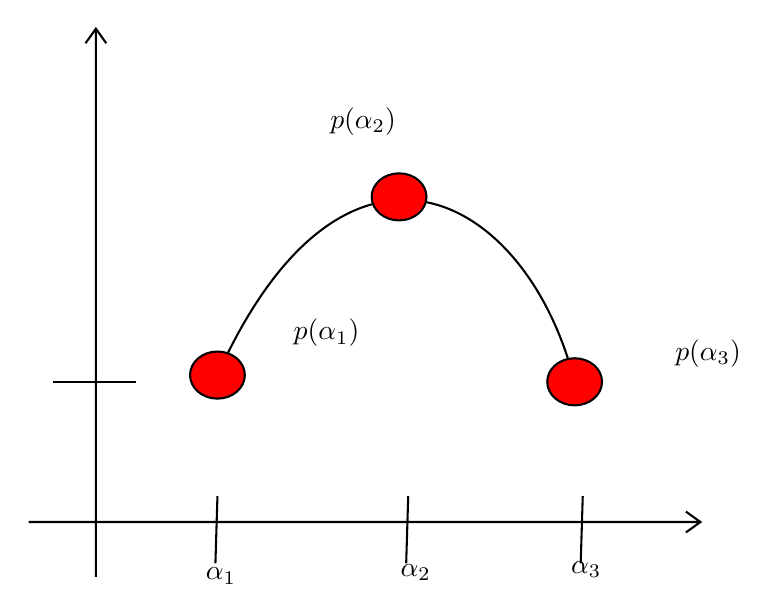
\begin{tikzpicture}[x=0.75pt,y=0.75pt,yscale=-1,xscale=1]
%uncomment if require: \path (0,300); %set diagram left start at 0, and has height of 300

%Shape: Axis 2D [id:dp4548434535748712] 
\draw  (156,247.67) -- (479.64,247.67)(188.36,10) -- (188.36,274.08) (472.64,242.67) -- (479.64,247.67) -- (472.64,252.67) (183.36,17) -- (188.36,10) -- (193.36,17)  ;
%Curve Lines [id:da9088123433049421] 
\draw    (246.93,176.87) .. controls (307.55,42.4) and (395.55,87.77) .. (419.02,180.11) ;
%Flowchart: Connector [id:dp8788809565179998] 
\draw  [fill={rgb, 255:red, 255; green, 0; blue, 0 }  ,fill opacity=1 ] (321.24,91.01) .. controls (321.24,84.74) and (327.15,79.67) .. (334.44,79.67) .. controls (341.73,79.67) and (347.64,84.74) .. (347.64,91.01) .. controls (347.64,97.27) and (341.73,102.35) .. (334.44,102.35) .. controls (327.15,102.35) and (321.24,97.27) .. (321.24,91.01) -- cycle ;
%Flowchart: Connector [id:dp8954838959032968] 
\draw  [fill={rgb, 255:red, 255; green, 0; blue, 0 }  ,fill opacity=1 ] (233.73,176.87) .. controls (233.73,170.61) and (239.64,165.53) .. (246.93,165.53) .. controls (254.22,165.53) and (260.13,170.61) .. (260.13,176.87) .. controls (260.13,183.14) and (254.22,188.22) .. (246.93,188.22) .. controls (239.64,188.22) and (233.73,183.14) .. (233.73,176.87) -- cycle ;
%Flowchart: Connector [id:dp6810968886330147] 
\draw  [fill={rgb, 255:red, 255; green, 0; blue, 0 }  ,fill opacity=1 ] (405.82,180.11) .. controls (405.82,173.85) and (411.73,168.77) .. (419.02,168.77) .. controls (426.31,168.77) and (432.22,173.85) .. (432.22,180.11) .. controls (432.22,186.38) and (426.31,191.46) .. (419.02,191.46) .. controls (411.73,191.46) and (405.82,186.38) .. (405.82,180.11) -- cycle ;
%Straight Lines [id:da6329359783579342] 
\draw    (167.73,180.11) -- (207.82,180.11) ;
%Straight Lines [id:da14731564882391568] 
\draw    (245.95,267.6) -- (246.93,235.2) ;
%Straight Lines [id:da2945881029344082] 
\draw    (337.86,267.6) -- (338.84,235.2) ;
%Straight Lines [id:da4835859670975893] 
\draw    (421.95,267.6) -- (422.93,235.2) ;

% Text Node
\draw (282.19,148.43) node [anchor=north west][inner sep=0.75pt]    {$p( \alpha _{1})$};
% Text Node
\draw (299.79,46.36) node [anchor=north west][inner sep=0.75pt]    {$p( \alpha _{2})$};
% Text Node
\draw (466.01,158.15) node [anchor=north west][inner sep=0.75pt]    {$p( \alpha _{3})$};
% Text Node
\draw (239.87,268.32) node [anchor=north west][inner sep=0.75pt]    {$\alpha _{1}$};
% Text Node
\draw (333.73,266.7) node [anchor=north west][inner sep=0.75pt]    {$\alpha _{2}$};
% Text Node
\draw (415.86,265.08) node [anchor=north west][inner sep=0.75pt]    {$\alpha _{3}$};


\end{tikzpicture}